\documentclass[12pt]{article}
\usepackage{amsmath}
\usepackage{amssymb}
\usepackage{amsfonts}
\usepackage{polski}
\usepackage{verbatim}
\usepackage{unicode-math}
\usepackage[utf8]{inputenc}
%\usepackage[polish]{babel}
\usepackage[T1]{fontenc}
\usepackage{graphicx}
%\usepackage[cp1250]{inputenc}
\usepackage{caption}
\usepackage{float}
\usepackage{enumitem}
\usepackage{hyperref}
\usepackage[output-decimal-marker={,}]{siunitx}

\title{Prognozowanie sezonowe - porównanie metod \\
    \large Teoria Algorytmów i Obliczeń \\}
\author{Piotr Widomski}
\date{02.01.2022}

\begin{document}

\maketitle

\section{Cel projektu}

Celem projektu jest porównanie wydajności prognozowania sezonowych szeregów czasowych za pomocą maszyny \texttt{SARIMA} (\texttt{Seasonal ARIMA}) oraz liniowej kombinacji maszyn \texttt{ARIMA} działających na co $n$-tym elemencie szeregu.

\section{Użyte dane}

Do porównania metod użyte zostały dane przedstawiające średnią miesięczną temperaturę powietrza mierzoną na dublińskim lotnisku od roku 1941. Dane zostały pobrane z portalu inicjatywy \href{https://data.gov.ie/dataset/dublin-airport-monthly-data?package_type=dataset}{Open Data} prowadzonej przez rząd irlandzki. Pomiary wykonane zostały przez \href{https://www.met.ie/}{Met Éireann} - irlandzki narodowy serwis meteorologiczny i udostępnione na licencji CC Attribution 4.0.

Na potrzeby projektu użyty został wycinek danych zawierających pełne lata, od 1942 do 2019 roku, czyli 78 lat pomiarów. Dane te zostały podzielone na treningowe oraz testowe w stosunku około $80\%$, gdzie dane treningowe zawierają 62 lata, od 1942 do 2003 roku, a dane testowe - 15 lat, od 2004 do 2019 roku. Rok 2021 został pominięty ze względu na niekompletność danych, natomiast 2020 - z powodu brakujących danych z marca.

\section{Opis metod}

\subsection{ARIMA}

\texttt{ARIMA} jest klasą modelów, które opisują szereg na podstawie poprzednich wartości. Model \texttt{ARIMA} składa się z trzech procesów:

\begin{itemize}
    \item \texttt{AR} (autoregresyjny) - każda wartość jest liniową kombinacją pewnej liczby poprzednich wartości. Liczbę poprzednich wartości użytych przy obliczeniu następnej oznaczamy przez $p$, a a proces autoregresyjny z rzędem regresji $p$ - \texttt{AR(p)} i przedstawiamy następująco:
          \[
              y_t = \alpha + \phi_1y_{t-1} + \phi_2y_{t-2} + \dots + \phi_py_{t-p} + \epsilon_t
          \]
          gdzie $y_{t-i}$ jest $i$-tą poprzednią wartością ciągu w chwili $t$, $\phi_i$ jest współczynnikiem i-tej poprzedniej wartości, $\epsilon_t$ zaburzeniem w momencie t, a $\alpha$ - wartością podstawową.
    \item \texttt{MA} (średniej ruchomej) - każda wartość jest zależna od zaburzenia w chwili obecnej oraz wcześniejszych. Liczbę poprzednich zaburzeń uwzględnionych przy obliczeniu następnej wartości oznaczamy przez $q$, a proces średniej ruchomej rzędu $q$ - \texttt{MA(q)} i przedstawiamy:
          \[
              y_t = \alpha + \epsilon_t + \theta_1\epsilon_{t-1} + \theta_2\epsilon_{t-2} + \dots + \theta_q\epsilon_{t-q}
          \]
          gdzie $\epsilon_t$ jest zaburzeniem w momencie t, $\theta_i$ - współczynnikiem $i$-tego poprzedniego zaburzenia, a $\alpha$ - wartością podstawową.
    \item \texttt{I} (integracja) - w celu modelowania ciągów niestacjonarnych, model \texttt{ARIMA} może wykonywać różnicowanie pewnego stopnia, w celu operowania na bardziej stacjonarnym ciągu. W takim wypadku, zamiast następnej wartości, model prognozuje różnicę wartości. Jednak dzięki znajomości poprzedniej wartości możemy wyliczyć na podstawie różnicy następną wartość. Stopień różnicowania oznacza się przez $d$.
\end{itemize}

Łącząc powyższe procesy, otrzymujemy ogólny wzór modelu \texttt{ARIMA}:
\begin{gather*}
    y_t^* = \alpha + \sum^p_{i=1}\phi_iy^*_{t-i} + \sum^q_{i=1} + \theta_i\epsilon_{t-i} + \epsilon_t \\
    y_t^* = \Delta^dy_t
\end{gather*}
Poszczególne modele \texttt{ARIMA} definiuje się za pomocą trzech zmiennych całkowitych $p, d, q$ i zapisuje \texttt{ARIMA(p, d, q)}.

\subsection{SARIMA}

\texttt{SARIMA}, lub \texttt{Seasonal ARIMA}, jest rozszerzeniem modelu \texttt{ARIMA} wspierającym ciągi czasowe wykazujące sezonowość, czyli takie, które posiadają powtarzające się z pewną określaną częstością zmiany wartości. Częstość tę oznaczymy przez $S$.

Rozszerzenie to dodaje trzy nowe, analogiczne do modelu \texttt{ARIMA} procesy:
\begin{itemize}
    \item Sezonową autoregresję - stopień oznaczamy przez $P$
    \item Sezonową średnią ruchomą - stopień oznaczamy przez $Q$
    \item Sezonową integrację - stopień oznaczamy przez $D$
\end{itemize}
W celu zdefiniowania wzoru modelu \texttt{SARIMA} zdefiniujmy operator poprzednika $B$:
\begin{gather*}
    By_t = y_{t-1} \\
    B^iy_t = y_{t-i}
\end{gather*}
Uwzględniając nowe procesy oraz operator $B$, otrzymujemy ogólny wzór modelu \texttt{SARIMA}:
\begin{gather*}
    \prod^p_{i=1}(1 - \phi_iB^i) \prod^P_{i=1}(1 - \Phi_iB^{Si}) \prod^d_{i=1}(1 - B^i) \prod^D_{i=1}(1 - B^{Si})y_t = \\
    \prod^q_{i=1}(1 + \theta_iB^i) \prod^Q_{i=1}(1 + \Theta_iB^{Si}) \epsilon_t
\end{gather*}

Poszczególne modele \texttt{SARIMA} definiuje się za pomocą zmiennych całkowitych niesezonowych $p, d, q$, zmiennych sezonowych $P, D, Q$ oraz częstości sezonowej $S$ i zapisuje \texttt{SARIMA(p, d, q) x (P, D, Q)S}.

\subsection{Kombinacja liniowa maszyn ARIMA}
\label{group-arima}

Model ten składa się z grup maszyn \texttt{ARIMA} działających na co $n$-tym elemencie ciągu z ostatnich $S$ elementów, gdzie $S$ jest częstością maszyny \texttt{SARIMA}. Każda z maszyn w grupie operuje na pewnym podciągu ciągu bazowego zawierającego co $n$-ty element ciągu. Podciągi te są parami rozłączne, oraz ich suma równa jest ciągowi bazowemu. Każdy podciągów w grupie jest równej długości. Z tego powodu narzucamy ograniczenie na $n$: $n|S$. Maszyny wewnątrz grupy są uporządkowane według kolejności podciągów, czyli za pierwszą uznajemy maszynę, której podciąg zaczyna się od pierwszego elementu ciągu, drugą - od drugiego, i tak dalej.

Weźmy grupy maszyn spełniające powyższe warunki i ponumerujmy je $1, 2, \dots, n$. Oznaczmy przez $y_{i,t}$ element otrzymany z grupy $i$ w momencie $t$. Wartość tą możemy uzyskać stosując wzór modelu \texttt{ARIMA} z maszyną z grupy $i$, której indeks wewnątrz grupy jest równy $t mod i$.
Stosując kombinację liniową maszyn \texttt{ARIMA} otrzymujemy następujący wzór na następny element:
\begin{gather*}
    y_t = \sum^n_{i=1}\alpha_iy_{i,t}
\end{gather*}
gdzie $\alpha_i$ jest współczynnikiem $i$-tej grupy. Model ten będzie również nazywany grupą maszyn \texttt{ARIMA} lub \texttt{ARIMA}.

\section{Implementacja}

\subsection{Biblioteka modeli}

Do budowy modeli została użyta biblioteka \href{https://www.statsmodels.org/stable/index.html}{\texttt{statsmodel}} zapewniająca implementacje modeli \texttt{ARIMA} oraz rozszerzenia \texttt{SARIMA}. Dodatkowo biblioteka ta umożliwia automatyczne dobranie odpowiednich współczynników na podstawie danych wejściowych oraz parametrów modelu. Dodatkowo udostępnia metody umożliwiające prognozowanie kolejnych elementów ciągu.

Dodatkowo, w celu dobrania optymalnych parametrów modeli, użyta została biblioteka \href{https://alkaline-ml.com/pmdarima/}{\texttt{pmdarima}}, która umożliwia wyszukanie optymalnych parametrów modelu na podstawie ustalonych kryteriów, po czym zwraca maszynę utworzoną z dobranych przez siebie parametrów w implementacji kompatybilnej z tą, która znajduje się w bibliotece \texttt{statsmodels}.

\subsection{SARIMA}

Przed konstrukcją modelu wykonana została analiza danych za pomocą algorytmu \href{https://www.statsmodels.org/stable/generated/statsmodels.tsa.seasonal.seasonal_decompose.html}{rozkładu sezonowego} udostępnionego przez bibliotekę \texttt{statsmodels}. Parametry modelu dobrane zostały zgodnie ze wskazówkami przedstawionymi przez \href{https://www.datasciencecentral.com/profiles/blogs/tutorial-forecasting-with-seasonal-arima}{Kostas Hatalis} Wynik rozkłądu prezentuje się następująco:

\begin{figure}[H]
    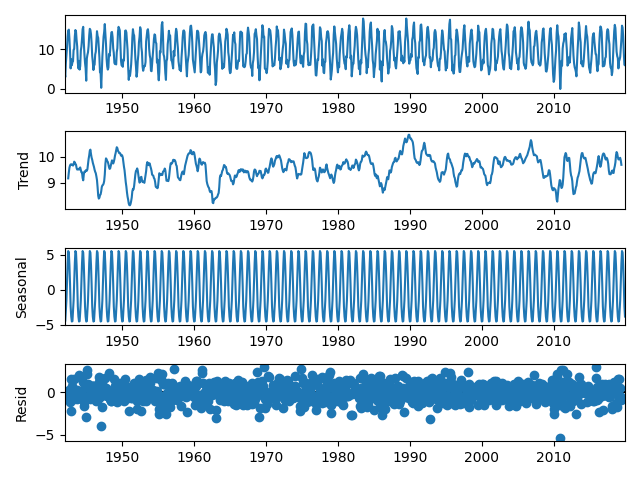
\includegraphics[width=\textwidth]{img/decomposition.png}
    \caption{Rozkład sezonowy danych}
\end{figure}

Wykres przedstawia kolejno: wartość, trend, komponent sezonowy oraz elemen losowy każdego elementu ciągu. W celu łatwiejszej analizy skupiono się na pierwszych dziesięciu latach:

\begin{figure}[H]
    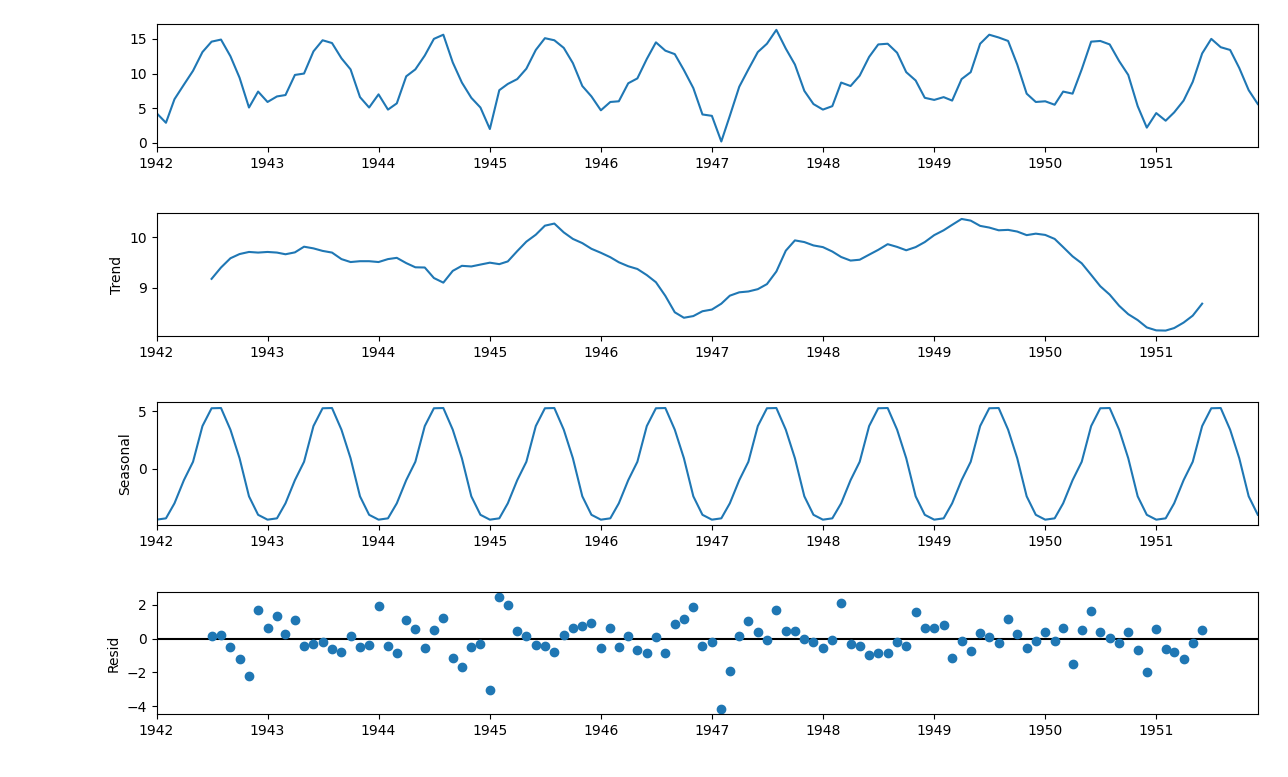
\includegraphics[width=\textwidth]{img/decomposition_10y.png}
    \caption{Rozkład sezonowy danych z pierwszych 10 lat}
\end{figure}

Z rozkładu danych zauważono, że zgodnie z oczekiwaniami dane posiadają stały element sezonowy o okresie wynoszącym dwanaście miesięcy. Element sezonowy jest stały, więc jako wartość parametru $D$ użyto $1$. Dodatkowo trend danych jest niejednoznaczny. Z tego powodu wartość parametru $d$ ustalono jako $0$.

Jako pomoc przy dobraniu pozostałych parametrów modelu \texttt{SARIMA} użyte zostały wykresy autokorelacji (ACF) oraz częściowej autokorelacji danych (PACF):

\begin{figure}[H]
    \begin{minipage}{.5\textwidth}
        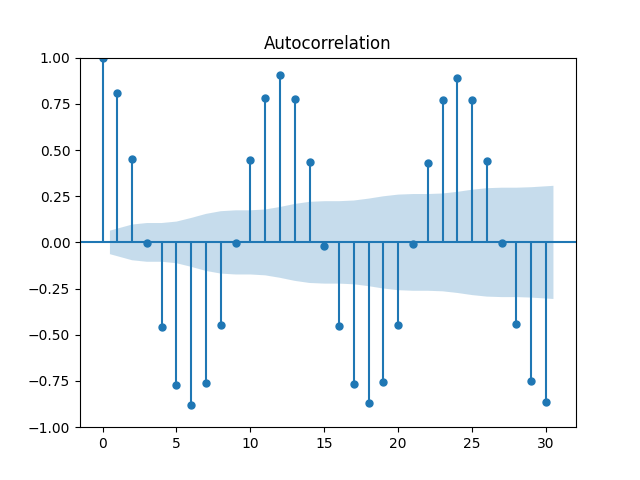
\includegraphics[width=\textwidth]{img/acf.png}
        \caption{Wykres autokorekacji}
    \end{minipage}
    \begin{minipage}{.5\textwidth}
        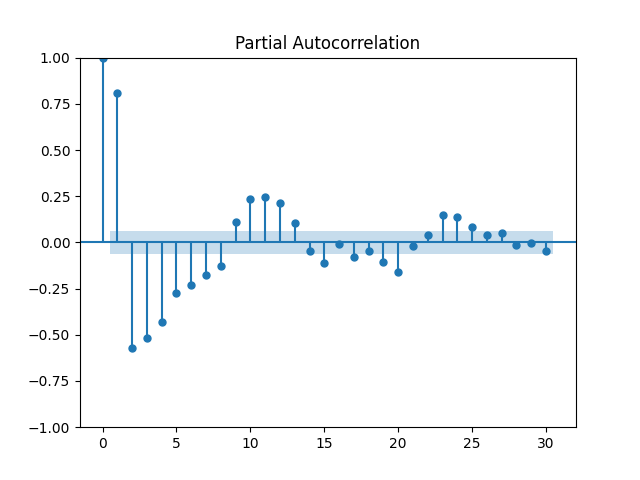
\includegraphics[width=\textwidth]{img/pacf.png}
        \caption{Wykres częsciowej autokorekacji}
    \end{minipage}
\end{figure}

Wykres ACF posiada największą wartość dla wartości $12, 24, \dots$, co potwierda hipotezę o sezonowej częstości wynoszącej $12$ miesięcy. Wykres przyjmuje wartości ponad poziomem istotności dla dwóch pierwszych wartości (pomijając zerową), co powoduje że jako parametr $q$ użyta została wartość $2$. Dodatkowo wartość dla elementu $12$, czyli $S$, jest dodatnia. Z tego powodu parametr $P$ będzie przyjmował wartość dodatnią, a parametr $Q$ - wartość $0$.

Wykres PACF przyjmuje wartości ponad poziomem istotności dla pierwszej wartości (pomijając zerową), co sprawia że jako parametr $p$ użyta została wartość $1$.

Na podstawie analizy danych model \texttt{SARIMA(1, 0, 2) x (P, 1, 0)12}. Dokładna wartość $P$ została dobrana przy użyciu metody automatycznego dobierania parametrów modelu udostępnionej przez bibliotekę \texttt{pmdarima} i wyniosła $2$. Zatem ostateczna postać modelu wyniosła \texttt{SARIMA(1, 0, 2) x (2, 1, 0)12}.

\subsection{ARIMA}

Grupa maszyn \texttt{ARIMA} została zaimplementowana zgodnie z \hyperref[group-arima]{opisem}, z grupami o $n$ równym odpowiednio $2, 3, 4$ i $6$. Definicja grupy mówi, że maszyny działają na co $n$-tym elemencie z ostatnich $S$. Dlatego też każda maszyna ma postać \texttt{ARIMA($\frac{S}{n}$, 0, $\frac{S}{n}$)}, gdzie $d = 0$ wynika z analizy przeprowadzonej podczas konstrukcji maszyny \texttt{SARIMA}. Podczas stosowania kombinacji liniowej wyników, z powodu bliskich wartości przewidywanych przez każdą z grup, jako współczynnik dla każdej grupy przyjęto wartość $\frac{1}{4}$.

\section{Wyniki}

Wyniki prezentują się następująco:

\begin{figure}[H]
    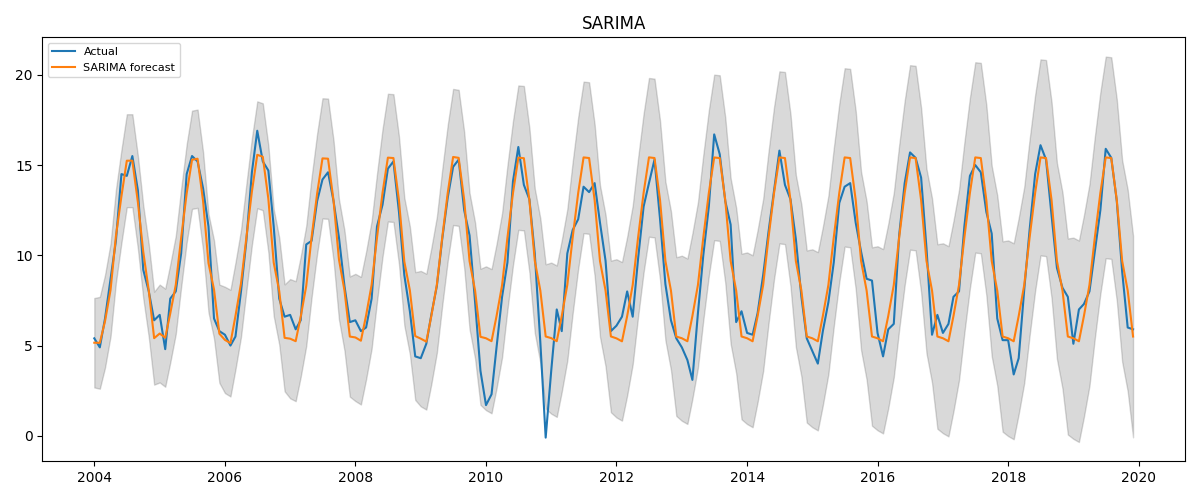
\includegraphics[width=\textwidth]{img/sarima.png}
    \caption{Wykres przewidywań modelu \texttt{SARIMA} z zaznaczoną pewnością $95\%$ oraz prawdziwych wartości}
\end{figure}

\begin{figure}[H]
    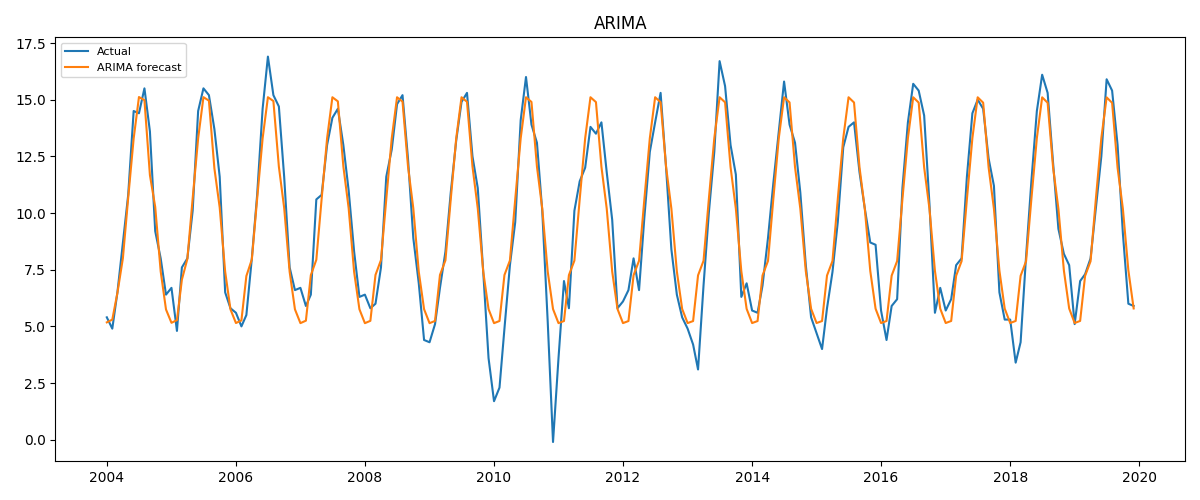
\includegraphics[width=\textwidth]{img/arima.png}
    \caption{Wykres przewidywań modelu kombinacji liniowej \texttt{ARIMA} oraz prawdziwych wartości}
\end{figure}

\begin{figure}[H]
    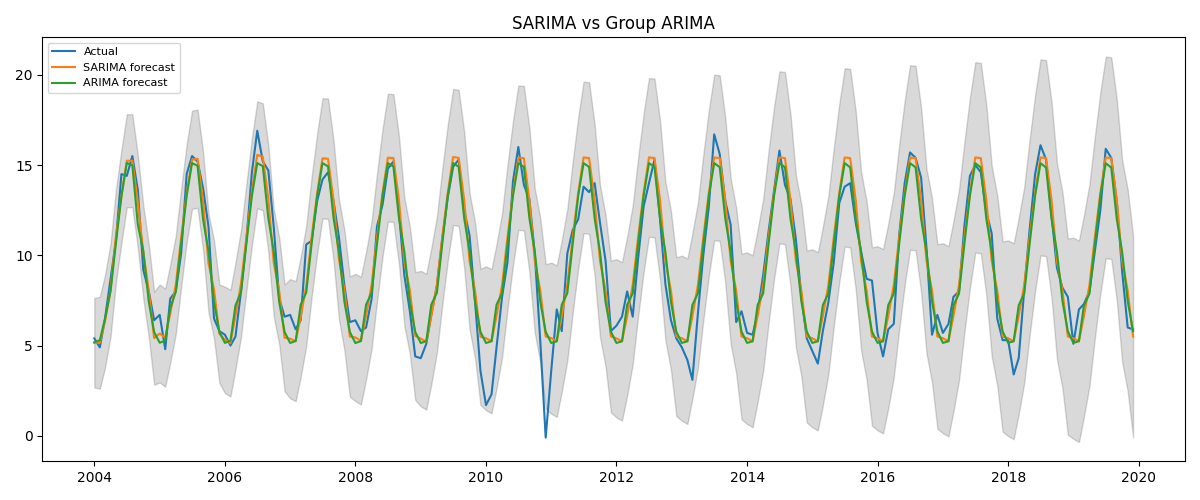
\includegraphics[width=\textwidth]{img/results.png}
    \caption{Wykres przewidywań obu modeli oraz prawdziwych wartości}
\end{figure}

\begin{figure}[H]
    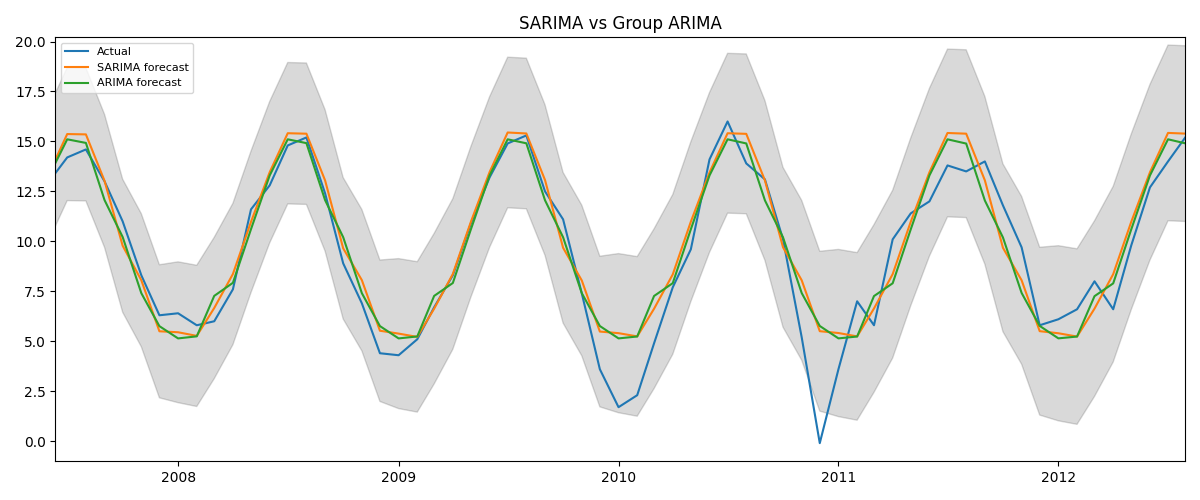
\includegraphics[width=\textwidth]{img/results_5y.png}
    \caption{Wykres przewidywań obu modeli oraz prawdziwych wartości przycięty do 5 lat}
\end{figure}

Model \texttt{SARIMA} osiągnął średni błąd kwadratowy równy $\num{1.2023}$ oraz średni błąd procentowy równy $\num{0.4212}$. Liniowa kombinacja maszyn \texttt{ARIMA} osiągnęła średni błąd kwadratowy równy $\num{1.2148}$ oraz średni błąd procentowy równy $\num{0.4346}$.

\newpage
\section{Wnioski}

Oba modele osiągnęły porównywalną efektywnośc oraz nie wykazują opóźnienia w zmianie trendu, co świadczy o świadomości sezonowej obu modeli. Jednocześnie wykresy obu modeli przypominają cykl, który nie wykazuje reakcji na nietypowe wartości, jak w przypadku przełomu 2009/2010 roku.

Przyglądając się wykresom można zauważyć, że model \texttt{SARIMA} posiada kształt bliższy wartościom rzeczywistym w okresie zimowym, kiedy wartości temperatury są najniższe i wachają się przez kilka miesięcy, przed ponownym wzrostem we wczesnej wiośnie. Natomiast model \texttt{ARIMA} lepiej przystosował się do wartości w okresie po nowym roku, gdzie często widzimy nagły skok, po którym następuje lekkie wygładzenie oraz ponowny wzrost.

Dobrane dane charakteryzują się niejednolitym trendem oraz niską względną różnicą wartości. Może to być jedna z przyczym obserwowanego zachowania danych.

\end{document}
